\title{Testing \LaTeX}
\author{Stefan Ehin\thanks{A student of University of Tartu}}
\date{\today}

\documentclass[12pt, letterpaper]{article}
\usepackage{graphicx}
\graphicspath{{../images}}

\begin{document}

\maketitle

\begin{abstract}
    This is a simple paragraph at the beginning of the 
    document. A brief introduction about the main subject.
\end{abstract}

\newpage

\tableofcontents  

\newpage

\section{Intro}

\textit{First document}. \textbf{This is a \textit{simple} example}, with \underline{no} 
extra parameters or packages included.

\section{Image}

\begin{figure}[h]
    \centering
    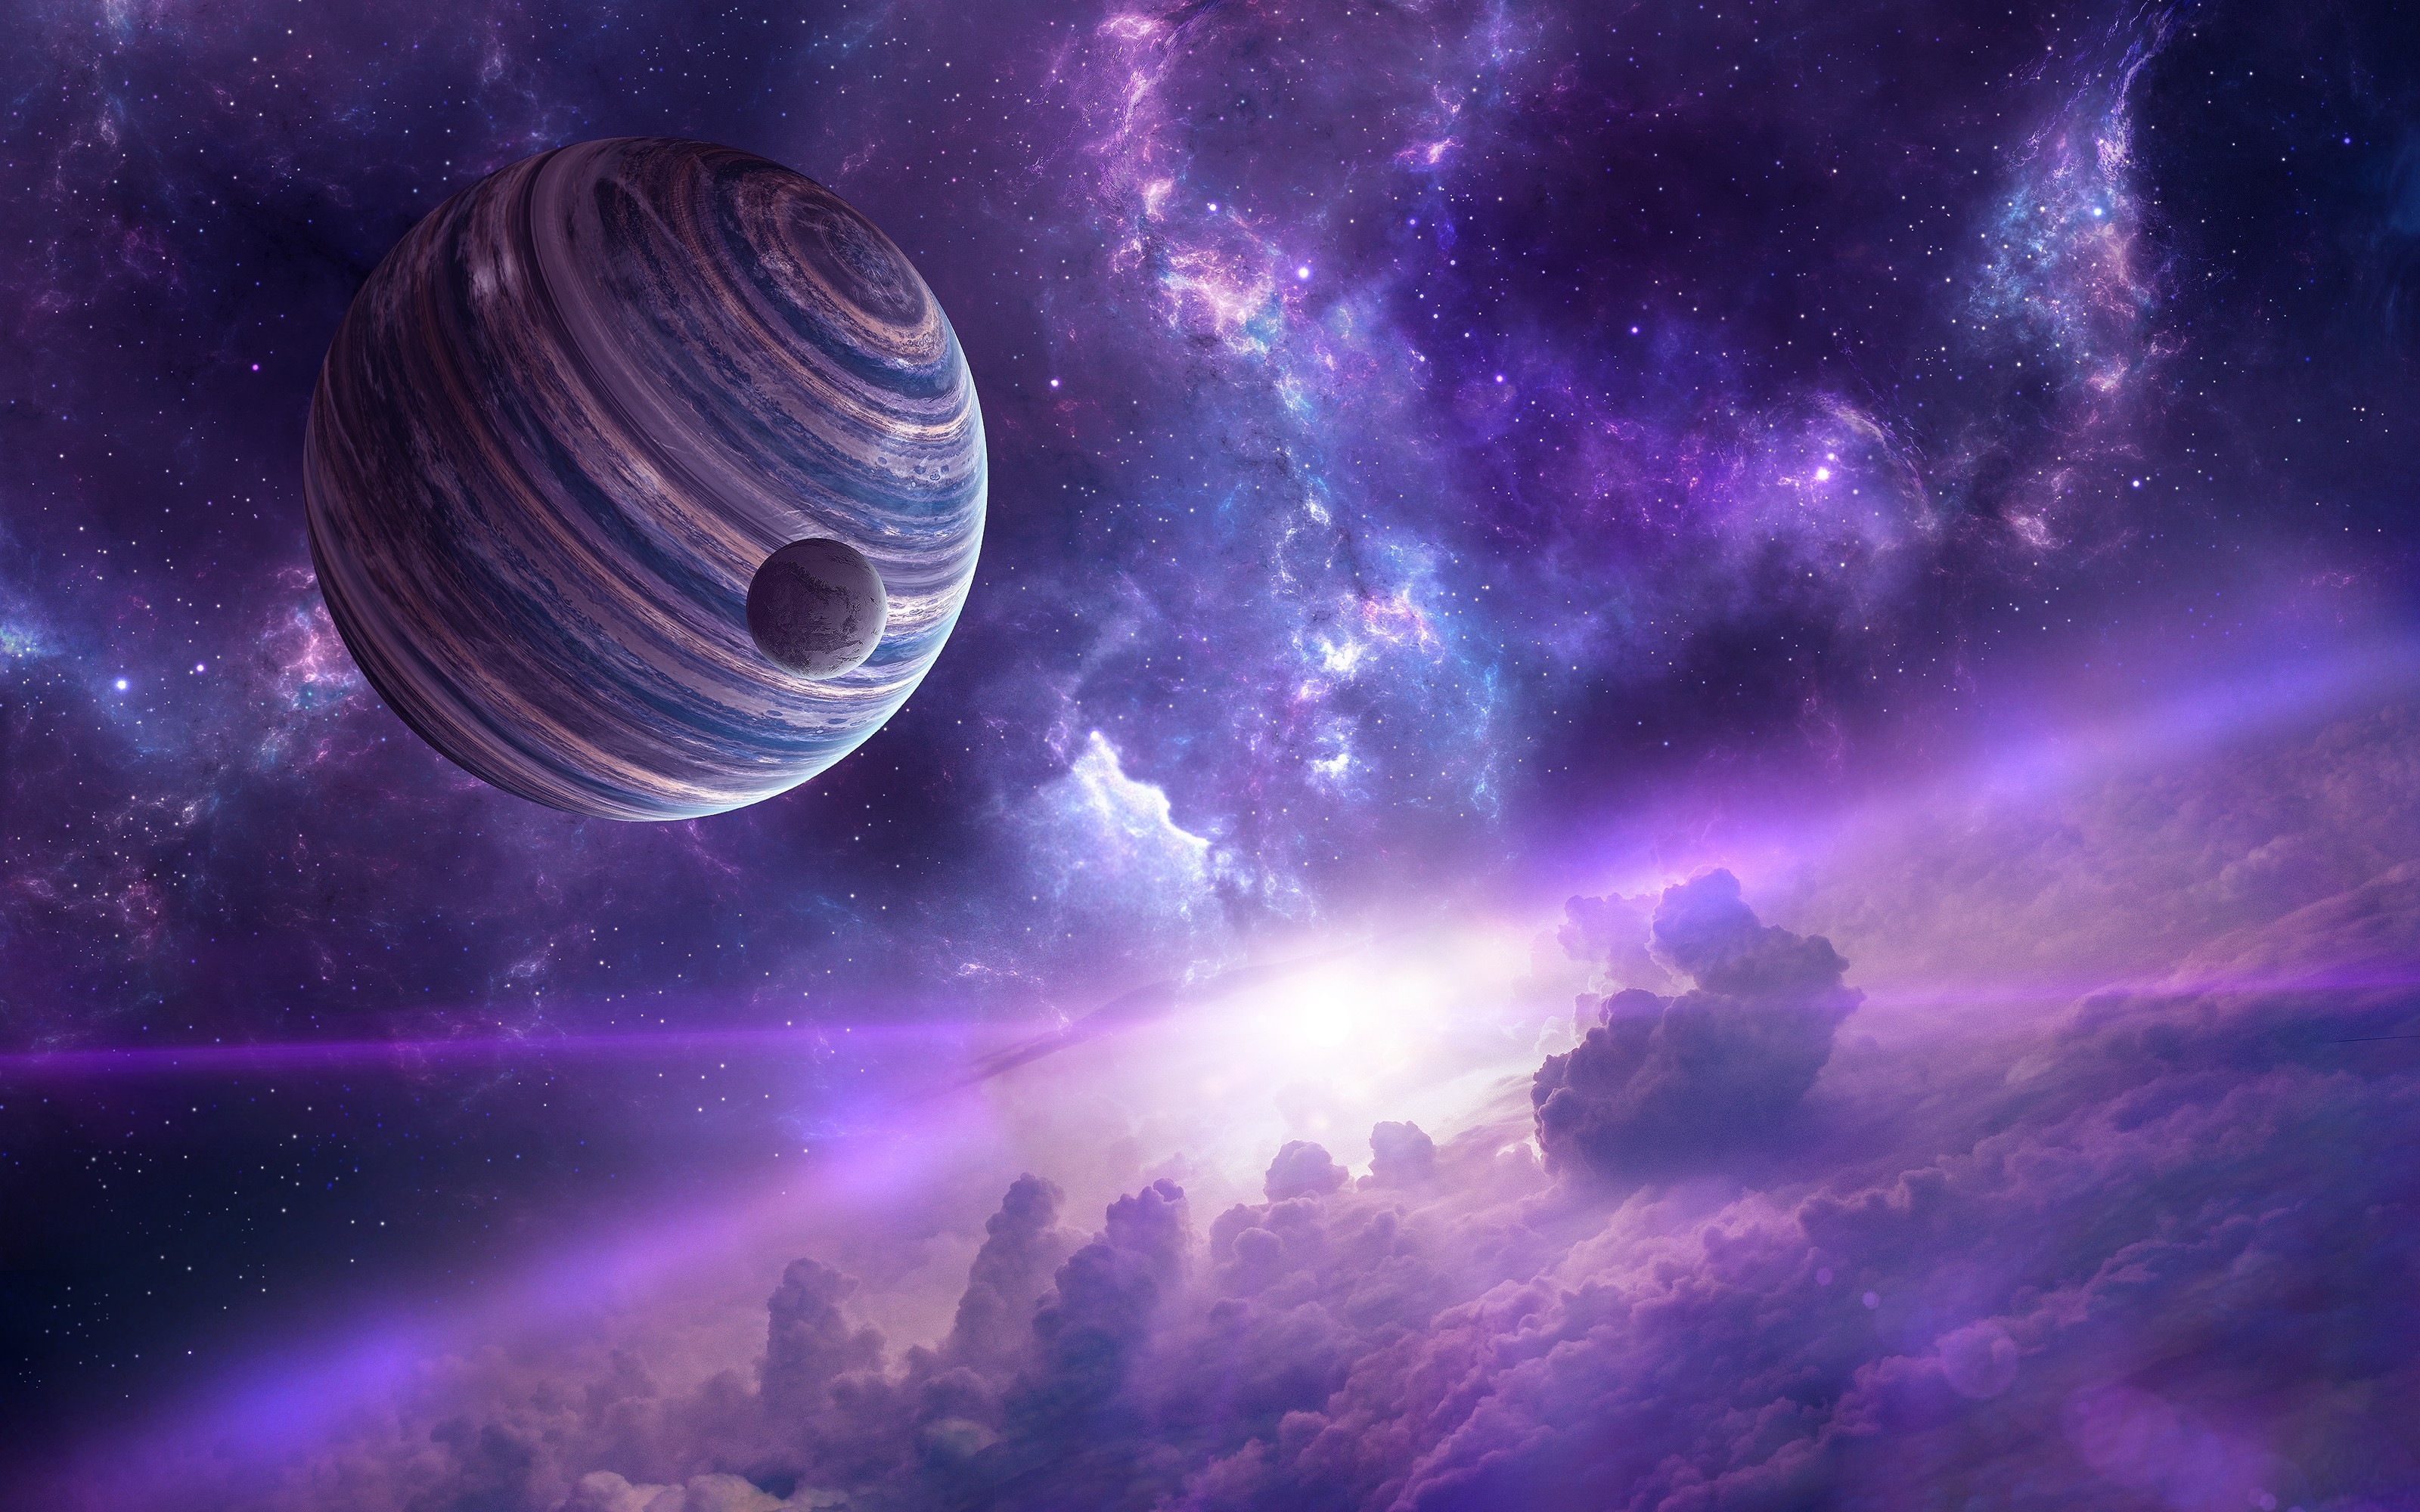
\includegraphics[width=0.70\textwidth]{universe.jpg}
    \caption{Our universe}
    \label{fig:universe}
\end{figure}

As we can see in the figure \ref{fig:universe} our universe is beautiful.

\section{List}

\begin{itemize}
    \item First 
    \item Second
    \item Third
\end{itemize}

\section{Math}

As Einstein once said: $E=mc^2$.

And as Newton used to say:

\[F=ma\]

And something else \dots

\[T^{i_0+1}_{i_0-1}\]

Need an integral? Easy: $\int$
Fraction? Huh: $\frac{a}{b}$

Ohh yu seem to like Greek don't you?

Well then: $\alpha$ $\omega$ $\epsilon$ $\varepsilon$
Not big enough?! Erh \dots
Take this: $\Delta$ $\Sigma$ $\Pi$ $\mathcal{E}$ $\mathcal{I}$

Love trig too?

\[\sin(-\alpha) = -\sin(\alpha)\]

\section{Tables}

\begin{table}
    \centering
    \begin{tabular}{c c c}
        a & b & c \\
        d & e & f \\
        g & h & i
    \end{tabular}
    \caption{Some table}
    \label{table:first-table}
\end{table}

\begin{table}
    \centering

    \begin{tabular}{c | c | c}
        o &   & x \\
        \hline
          & o & x \\
        \hline
          & x & o
    \end{tabular}
\tableofcontents  
\caption{You know what it is \dots}
    \label{table:tic-tac-toe}
\end{table}

Is it table \ref{table:tic-tac-toe} just a tic-tac-toe table?!

\end{document}